
\documentclass[12pt, a4paper]{article}

\usepackage[utf8]{inputenc}
\usepackage[T1]{fontenc}
\usepackage[russian]{babel}
\usepackage[oglav,spisok,boldsect,eqwhole,figwhole,hyperref,hyperprint,remarks,greekit]{./style/fn2kursstyle}
\graphicspath{{./style/}{./figures/}}
\usepackage{color,soul}
\usepackage{multirow}
\usepackage{supertabular}
\usepackage{multicol}
\usepackage{subcaption}
\usepackage{float}
\usepackage{xcolor,colortbl}
\definecolor{Gray}{gray}{0.87}
% Параметры титульного листа
\title{Задача об ограниченном ранце}
\author{Г.\,А.~Швецов}
\supervisor{А.\,Ю.~Попов}
\group{ФН2-42Б}
\date{2022}

% псевдокод
% https://harrix.dev/blog/2013/algorithmicx-cyrillic/
\usepackage{algorithm}
\usepackage[noend]{algpseudocode}
\newcommand{\algorithmicbreak}{\textbf{break}}
\newcommand{\Break}{\State \algorithmicbreak}

\usepackage{comment}

% Переопределение команды \vec, чтобы векторы печатались полужирным курсивом
%\renewcommand{\vec}[1]{\text{\mathversion{bold}${#1}$}}%{\bi{#1}}
%\newcommand\thh[1]{\text{\mathversion{bold}${#1}$}}
%Переопределение команды нумерации перечней: точки заменяются на скобки
\renewcommand{\labelenumi}{\theenumi)}

% Кастомный список вида Шаг *.
\usepackage{enumitem}
\newlist{STEP}{enumerate}{1}
\setlist[STEP]{label=\textbf{Шаг \arabic*.}, leftmargin=1.75cm}

% TODO в конце пройтись по оформлению текста, например, чтобы строка не заканчивалась на однобуквенный союз или предлог или чтобы последняя строка абзца была в 1,5 раза длиннее красной строки

\begin{document}
	
	\maketitle
	
	\tableofcontents
	
	\newpage
	
	\section-{Введение}
	
	Классическая задача о рюкзаке (о загрузке) известна очень давно, и формулируется следующим образом. Пусть есть $n$ разных предметов, каждый предмет имеет вес $w_i$ и полезность $c_i$, так же имеется максимальный вес $W$, который можно положить в рюкзак. Требуется собрать такой набор предметов, чтобы полезность их была наибольшей, а суммарный вес не превышал $W$. Несмотря на такую "бытовую"\, формулировку, решение данной задачи находит гораздо более широкое применение.
	
	% https://docs.yandex.ru/docs/view?url=http%3A%2F%2Falgoritm-rukzaka.narod.ru%2Fo_rjukzake.pdf
	% На основе задачи о ранце был разработан первый алгоритм шифрования с открытым ключом --- https://habr.com/ru/post/529346/ 
	Задача о загрузке (или задача о рюкзаке) и различные ее модификации широко применяются на практике в прикладной математике, криптографии, экономике, логистике, для нахождения решения оптимальной загрузки различных транспортных средств: самолетов, кораблей, железнодорожных вагонов и т.д. Приведем в качестве примера задачу, которая представляет собой переиначенную задачу о ранце, чтобы показать, что алгоритмы для решения данной проблемы могут быть полезны не только в упаковке багажа:
	
	% TODO сослаться на файл Book-advanced-algorithms.pdf с trello, находится на странице 98
	Технология \emph{DVS}\footnote{DVS (от англ. Dynamic Voltage Scaling) --- динамическое изменение напряжения.} позволяет снижать напряжение на процессоре и добиваться экономии электроэнергии за счет увеличения времени выполнения задачи.
	
	Пусть процессор поддерживает два уровня напряжения --- $U_L < U_H$. Есть набор из $n$ задач, каждая из которых имеет энергоемкость и время выполнения для обоих режимов, т.е. для $i=1, \dots, n$ даны энергоемкости $c_i^H$ и $c_i^L$ и длительности $t_i^H$ и $t_i^L$.
	
	Нужно выполнить все задачи на одном процессоре за время не более заданного~$T$, при этом добиться минимального энергопотребления.
	
	\medskip
	
	Рассматриваемая нами задача является $N\!P$-полной, то есть для нее не существует полиномиального алгоритма, решающего ее за разумное время, в этом и заключается основная проблема данной задачи. Решения $N\!P$-полных задач обычно делят на два типа: приближенные, работающие быстро, но далеко не всегда решающие задачу наилучшим образом, и точные, выполняемые сильно дольше, но гарантированно выдающие лучший результат.
	
	% https://neerc.ifmo.ru/wiki/index.php?title=Задача_о_рюкзаке
	Существует несколько модификаций задачи о ранце. Ниже приведены некоторые из них.
	\begin{enumerate}
		\item Каждый предмет можно брать только один раз.
		\item Каждый предмет можно брать сколько угодно раз.
		\item Каждый предмет можно брать определенное количество раз.
		\item Можно брать дробную часть предмета.
	\end{enumerate}
	
	\medskip
	\underline{Цель данной работы} --- реализовать решение для задачи 3) двумя точными алгоритмами, а именно методом ветвей и границ и динамическим программирова\-нием, на языке программирования C++ и в системе компьютерной алгебры Wolfram Mathematica. Также исследовать время выполнения и сложность алгоритмов.
	
	\section{Постановка задачи}
	
	Математически задачу об ограниченном рюкзаке можно представить следующим образом:
	\begin{equation}
		\label{problem}
		\begin{gathered}
			\sum_{i=1}^{n} c_i x_i \rightarrow \max, \\
			\sum_{i=1}^{n} w_i x_i \le W, \\
			x_i \in \{0,1,\dots,k_i\},
		\end{gathered}
	\end{equation}
	где $c_i$, $w_i$ и $k_i$ --- стоимость, вес и максимальное количество предмета $i$ соответственно; $W$ --- максимальная грузоподъемность ранца; $n$ --- количество предметов.
	
	Очевидно, что сложность алгоритма, осуществляющего полный перебор, т.е. проверяющего всевозможные наборы предметов, пропорциональна количеству этих возможные наборов. Таким образом он имеет сложность $O(K^n)$, где $K = \max\limits_{i=1,\dots,n} k_i$, что очень неэффективно. Поэтому, как и во многих других задачах, есть методы решения задачи, которые выполняются быстрее обычного перебора.
	
	\section{Метод ветвей и границ}
	
	Метод ветвей и границ (МВГ) относится к числу основных методов решения задач оптимизации. Этот метод основан на древовидной декомпозиции исходной задачи на подзадачи.
	
	В процессе дальнейшего изложения мы будем употреблять термин рекорд, означающий наилучшее найденное значение целевой функции (функции подлежащей оптимизации) к данному шагу алгоритма. Предполагается, что рекорд, также как и~целевая функция, принимает действительные значения.
	
	Различные варианты МВГ имеют специфичные для решаемой задачи особенности, но при этом подчиняются следующей общей схеме \cite{Kolpakov}:
	
	\textbf{Данные:} рекорд, список подзадач.
	
	\begin{STEP}
		\item В список подзадач помещается исходная задача.
		\item Если список подзадач пуст, то завершить алгоритм. В противном случае из списка выбирается и удаляется подзадача $P$.
		\item Вычисляется значение целевой функции, и при необходимости обновляется значение рекорда. Для задачи $P$ проверяется выполнимость условия отсева. Если подзадача $P$ удовлетворяет условию отсева, то осуществляется переход к шагу 2.
		\item Задача $P$ подвергается декомпозиции. Полученные в результате подзадачи помещаются в список подзадач. Перейти к шагу 2.
	\end{STEP}
	
	Т.е. конкретный вариант метода ветвей и границ определяется следующими тремя функциями: выбором подзадачи из списка; условием отсева; правилом декомпозиции, определяющим, каким образом разбивается очередная подзадача.
	
	Опишем данные функции для задачи об ограниченном ранце.
	
	Для начала запишем линейную задачу релаксации (т.е. задачу с ослабленным условием), соответствующей задаче \eqref{problem}:
	\begin{equation}
		\label{relax_problem}
		\begin{gathered}
			\sum_{i=1}^{n} c_i x_i \rightarrow \max, \\
			\sum_{i=1}^{n} w_i x_i \le W, \\
			0 \le x_i \le k_i.
		\end{gathered}
	\end{equation}
	
	Оптимум (оптимальное значение) задачи \eqref{relax_problem} не меньше оптимума исходной задачи \eqref{problem}. Задача релаксации представляет собой одномерную задачу линейного программирования и может быть решена \textit{методом Данцига}\footnote{Джордж Бернард Д\'{a}нциг (англ. George Bernard Dantzig; 8 ноября 1914 -- 13 мая 2005) --- американский математик, основоположник линейного программирования, известен как разработчик алгоритма, применяемого в решениях задач симплекс-методом.} следующим образом. Переменные нумеруются в порядке возрастания удельной стоимости:
	\[
	\frac{c_1}{w_1} \ge \dots \ge \frac{c_n}{w_n}.
	\]
	
	Сначала определяется номер $s$ дробной переменной по следующему правилу:
	\[
	s = \min \left\{j \in \{1,\dots, n\} : \sum_{i=1}^j k_i w_i > W \right\}.
	\]
	
	Таким образом решение состоит из предметов $i = 1, \dots, (s-1)$ в количестве $k_i$ и~предмета $s$ в количестве
	\[
	K = \frac{W - \sum\limits_{i=1}^{s-1} k_i w_i}{w_s},
	\]
	а стоимость итогового набора задачи \eqref{relax_problem}
	\[
	S = \sum_{i=1}^{s-1} k_i c_i + K\cdot c_s.
	\]
	
	Данный алгоритм имеет сложность $O(n)$. На основании данного решения введем функцию $S(i, w)$, решающую аналогичную задачу для предметов $j = i,\dots, n$ и вместимости рюкзака $w$, т.е. $S$, определенное выше, для задачи \eqref{relax_problem} есть значение $S(1, W)$.
	
	Теперь сформулируем, что будем понимать под подзадачей в рамках загрузки рюкзака. Пусть мы зафиксировали количество у первых $m$ предметов. Данный набор имеет стоимость $C'$ и вес $W'$. Тогда под подзадачей будем называть следущее:
	\begin{equation}
		\label{subproblem}
		\begin{gathered}
			C' + \sum_{i=m+1}^{n} c_i x_i \rightarrow \max, \\
			\sum_{i=m+1}^{n} w_i x_i \le W - W', \\
			x_i \in \{0,1,\dots,k_i\} \textrm{ при } i=(m+1),\dots, n.
		\end{gathered}
	\end{equation}
	
	Теперь мы готовы, наконец, сформулировать три функции, характеризующие метод ветвей и границ.
	
	\textit{Правило декомпозиции.} Исходную подзадачу \eqref{subproblem} будем разбивать на $(k_{m+1}+1)$ подзадач, фиксируя в каждой новой такой задаче предмет $(m + 1)$ в количестве $0, 1, 2, \dots, k_{m+1}$ штук. Отметим, что если в подзадаче \eqref{subproblem} присутствует всего один предмет $n$, то нет смысла разбивать ее на подзадачи, потому что мы можем сразу дать на нее ответ.
	
	% идею с жадным алгоритом я взял со stack overflow
	\textit{Выбор подзадачи из списка.} В основном, выбор подзадачи можно сделать произвольным, но мы будем пользоваться логикой жадных алгоритмов. Чтобы задача релаксации выполнялась за $O(n)$ необходимо, чтобы предметы изначально были отсортированы по убыванию удельной стоимости, поэтому будем предполагать, что предметы изначально отсортированы. Таким образом можно предположить, что нам выгодней взять как можно больше первых предметов. Поэтому после декомпозиции мы сначала будем рассматривать задачу при условии, что мы взяли предмет $(m+1)$ в количестве $k_{m+1}$, потом $(k_{m+1} - 1)$ и т.д.
	
	\textit{Условие отсева.} Подзадача не подлежит дальнейшей декомпозиции если:
	\begin{enumerate}
		\item подзадача не имеет решения, что возможно только при условии $W' < 0$;
		\item оптимум задачи \eqref{relax_problem} не превосходит значения рекорда (тогда, как было отмечено выше, оптимум задачи \eqref{subproblem} тоже не превосходит значения рекорда).
	\end{enumerate}
	
	Сложность алгоритма метода ветвей и границ составляет, как и при использовании перебора,~$O(K^n)$, где $K = \max\limits_{i=1,\dots,n} k_i$, т.к. в худшем случае условие отсева не сработает ни разу и мы будем вынуждены рассмотреть все возможные варианты.
	
	\section{Реализация метода ветвей и границ}
	
	\subsection{Особенности реализации на языке C++}
	Стандартная библиотека C++ предоставляет удобный контейнер для хранения и обработки различных структур данных --- std::vector<T>. Для удобства представления предметов рюкзака создана структура Item в отдельном заголовочном файле Item.h. При инициализации она получает имя предмета (name), его количество (count), вес (weight) и стоимость (cost). 
	
	Решение исходной задачи методом перебора представлено для пользователя функцией BranchAndBoundMethod::problemSolve, принимающей на вход вектор предметов items и вместимость рюкзака max\_weight. Задача данной функции подготовить данные для основной функции МВГ find\_bests, а именно отсортировать список предметов items по убыванию удельной стоимости.
	
	Функция find\_bests, принимающая на вход вместимость рюкзака и два итератора: на первый и последний рассматриваемые предметы. В целом она повторяет расписанный ход действий, описанный в предыдущем разделе. Для оценки сверху, \looser{-0.02}{т.е. условия отсева, реализована функция find\_best\_greedily, так же использующая два итератора и вместимость в качестве входных данных и реализующая метод Данцига.}
	
	Также в процессе работы были реализованы вспомогательные функции для отладки и работы с файлами: generateItems --- генерирует случайный набор предметов, FileToVector --- читает из файла массив, VectorToFile --- соответственно записывает массив в файл.
	
	\subsection{Особенности реализации на Wolfram Mathematica}
	Встроенные возможности системы Wolfram Mathematica значительно упрощают решение данной задачи, в особенности при обработке данных. Для работы с файлами использовались в основном такие команды, как SetDirectory (задание директории) и~Import, для работы с List --- команды AppendTo, MapIndexed и SortBy (добавление в конец, преобразование с учетом индекса и сортировка по правилу соответственно), для замера времени --- Timing. \looser{-0.02}{Кроме того, использовались программные блоки (Block) для реализации алгоритма с созданием временных переменных.}
	
	Также были реализованы пользовательские функции findBestGreedly и findBest, с~помощью которых осуществляются оценка сверху и поиск решения соответственно. Метод ветвей и границ реализован в виде пользовательской функции babMethod, принимающей на вход вместимость рюкзака (maxWeight) и список предметов (items).
	
	\section{Метод динамического программирования}
	% https://ru.m.wikipedia.org/wiki/Динамическое_программирование
	Словосочетание "динамическое программирование"\, впервые было использовано в 1940-х годах \textit{Ричардом Беллманом}\footnote{Ричард Эрнест Б\'{е}ллман (26 августа 1920, Нью-Йорк, США -- 19 марта 1984, Лос-Анджелес, США) --- американский математик, один из ведущих специалистов в области математики и вычислительной техники. Член Национальной инженерной академии США (1977), Национальной академии наук США (1983).} для описания процесса нахождения решения задачи, где ответ на одну задачу может быть получен только после решения задачи, "предшествующей"\, ей. В 1953 году он уточнил это определение до современного. Вклад Беллмана в динамическое программирование был увековечен в названии уравнения Беллмана, центрального результата теории динамического программирования, который переформулирует оптимизационную задачу в рекурсивной форме.
	% TODO можно добавить формулу Белмана
	
	Слово "программирование"\, в словосочетании "динамическое программирование"\, в действительности к "традиционному"\, программированию (написанию кода) почти никакого отношения не имеет. Слово "программа"\, в данном контексте скорее означает оптимальную последовательность действий для получения решения задачи. К~примеру, определенное расписание событий на выставке иногда называют программой.
	
	Динамическое программирование --- способ решения сложных задач путем разбиения их на более простые подзадачи. Ключевая идея в динамическом программировании достаточно проста. Как правило, чтобы решить поставленную задачу, требуется решить отдельные части задачи (подзадачи), после чего объединить решения подзадач в одно общее решение. Часто многие из этих подзадач одинаковы. Подход динамического программирования состоит в том, чтобы решить каждую подзадачу только один раз, сократив тем самым количество вычислений. Это особенно полезно в случаях, когда число повторяющихся подзадач экспоненциально велико.
	
	Чтобы успешно решить задачу динамикой нужно \cite{habr}:
	\begin{enumerate}
		\item состояние динамики: параметры, однозначно задающие подзадачу;
		\item значения начальных состояний;
		\item переходы между состояниями: формула пересчета;
		\item порядок пересчета;
		\item положение ответа на задачу: иногда это сумма или, например, максимум из значений нескольких состояний.
	\end{enumerate}
	
	Для решения нашей задачи введем двумерный массив $dp$ размером $n+1$ на $W+1$, где в $dp[i, w]$ будем хранить максимально возможную стоимость набора состоящая из первых $i$ предметов при максимальной допустимой нагрузке $w$. Теперь распишем пункты выше.
	\begin{enumerate}
		\item состояние динамики: $dp[i, w]$;
		\item начальные состояния: $dp[0, w]$ и $dp[i, 0]$ равны нулю, т.е. если у нас нет никаких вещей или мы не можем ничего положить в рюкзак, то и максимально возможная стоимость равна нулю;
		\item формула пересчета: $dp[i, w] = \!\max\limits_{x_j = 0,1,\dots, m(i,w)} \left(x_j\cdot c_i + dp[i-1, w - x_j\cdot w_i]\right)$, где \linebreak $m(i, w)$ --- максимальное количество предмета $i$, которое влезает в рюкзак вместимости $w$, ограниченное при этом максимальным количеством $k_i$, таким образом $m(i, w) = \min\left\{k_i;\; \left\lfloor\sfrac{w}{w_i}\right\rfloor\right\}$;
		\item пересчитывать будем в следующем порядке: для каждого $i$ будем заполнять строку $dp[i, w]$, $w$ изменяется в диапазоне от 1 до $W$, т.е. постепенно будем добавлять каждый предмет по порядку;
		\item ответ будет находится в ячейке $dp[n, W]$, т.к. это именно та задача, которую нам надо решить, для всех $n$ предметов при емкости рюкзака $W$.
	\end{enumerate}
	
	Таким образом, заполнение массива $dp$ можно представить в виде следующего псевдокода \cite{ITMO}:
	\begin{algorithmic}[1]
		\For{$w=0 \textbf{ to } W$}
		\State $dp[0, w] = 0$
		\EndFor
		
		\For{$i=1 \textbf{ to } n$}
		\For{$w=1 \textbf{ to } W$}
		\State $dp[i, w] = dp[i-1, w]$
		\For{$x_j = \min\left\{k_i, \left\lfloor\sfrac{w}{w_i}\right\rfloor\right\} \textbf{ downto 1}$}
		\State $dp[i, w] = \max\Big\{dp[i, w];\;\, x_j\cdot c_i + dp[i-1, w - x_j\cdot w_i]\Big\}$
		\EndFor
		\EndFor
		\EndFor
	\end{algorithmic}
	
	% взято отсюда https://algorithmica.org/tg/knapsack-gis-gcs
	\looser{-0.02}{Такое решение работает за $O(n\,W^2)$, так как $k_i$ могут быть очень большими, а $w_i = 1$.}
	
	% TODO можно вставить сюда таблицу 1.5 из файла mdo2p.pdf, как пример заполненной таблицы dp, ну и плюс уже будет не чисто текст, а с какой-то графикой
	
	Теперь опишем восстановление одного из решений также в виде псевдокода.
	\begin{algorithmic}[1]
		\State $w = W$
		\State $solution = \{\;\}$
		\For{$i=n \textbf{ downto } 1$}
		\If{$w = 0$}
		\Break
		\EndIf
		\State \parbox[t]{\dimexpr12cm-\algorithmicindent}{Находим $mVal = \max\limits_{x_j = 0,1,\dots, m(i,w)} \left(x_j\cdot c_i + dp[i-1, w - x_j\cdot w_i]\right)$ и $mCnt = x_j$, на котором достигается $mVal$}
		\If{$mCnt \ne 0$}
		\State \parbox[t]{\dimexpr11.5cm-\algorithmicindent}{Добавляем в решение $solution$ предмет $i$ в количестве $mCnt$ штук}
		% эти страшные команды нужны для красивого знака -=
		\State $w\,\,\scalebox{0.75}[1.0]{\(-\)}\!\!=\, w_i \cdot mCnt$
		\EndIf
		\EndFor
	\end{algorithmic}
	
	Впоследствии выполнения алгоритма итоговое решение будет представлено массивом $solution$. Сложность алгоритма восстановления одного решения составляет $O(n)$, потому что в общем случае мы пройдем по всем $n$ предметам.
	
	В итоге алгоритм имеет временную сложность $O(n\,W^2)$, а по памяти $O(n\,W)$, которая требуется на хранение массива $dp$. Также заметим, что если требуется найти только максимальную стоимость набора, не восстанавливая само решение, то потребление памяти можно сократить до $O(W)$, храня только две последние рассматриваемые строчки.
	
	\section{Реализация метода динамического программирования}
	
	\subsection{Особенности реализации на языке C++}
	Реализация полностью совпадает с псевдокодом алгоритма, указанного в предыдущем разделе. Но благодаря широким возможностям управления памятью в языке программирования C++ удалось увеличить быстродействие и уменьшить потребление	памяти. Некоторые вспомогательные функции, например, для работы с файлами и генерации предметов были заимствованы из реализации метода ветвей и границ на языке C++.
	
	\subsection{Особенности реализации на Wolfram Mathematica}
	Как и в случае с МВГ, возможности системы очень полезны при выполнении данной задачи. Встроенные команды позволили значительно сократить объем написанного кода, устранив необходимость в создании большого числа пользовательских функций. Большая часть команд, указанных в описании реализации метода перебора, нашли применение и в данном алгоритме. В процессе выполнения практики были реализованы пользовательские функции, необходимые для данного метода, такие как dynamic и dynFindAns, выполняющие заполнение матрицы $dp$ и восстановление решений соответственно.
	
	\section{Примеры работы программ}
	Приведем некоторые примеры решения задачи о рюкзаке на языке программирования С++ и в системе компьютерной алгебры Wolfram Mathematica. Исходные данные и результаты выполнения представлены в таблицах \eqref{tab:example1}, \eqref{tab:example2} и \eqref{tab:example3}. Названия заголовков таблиц имеют тот же смысл, что и в описании особенностей реализации метода ветвей и границ на языке программирования C++. Первый пример представляет собой задачу ранца 0-1, т.к. количество каждого предмета ограничено единицей. Дополнительно отметим, что задача, описанная в таблице \eqref{tab:example3}, имеет два решения.
		\begin{table}[H]
		\small
		\centering		
		\caption{Пример при вместимости рюкзака $\textrm{max\_weight}=1500$}\medskip
		\begin{tabular}{|c|c|c|c|}
			\hline
			\multicolumn{4}{|c|}{\textbf{Исходные данные}}\\
			\hline
			\rowcolor{Gray}
			item & count & weight & cost \\
			\hline
			1 & 1 & 200 & 40 \\
			\hline
			2 & 1 & 314 & 50 \\
			\hline
			3 & 1 & 198 & 100 \\
			\hline
			4 & 1 & 500 & 60 \\
			\hline
			5 & 1 & 200 & 30 \\
			\hline
			6 & 1 & 400 & 45\\
			\hline
		\end{tabular}
		\qquad
		\begin{tabular}{|c|c|c|c|}
			\hline
			\multicolumn{4}{|c|}{\textbf{Решение}}\\
			\hline
			\rowcolor{Gray}
			item & count & max\_cost & sum\_weight \\
			\hline
			5 & 1 & \multirow{5}{*}{\large 265} & \multirow{5}{*}{\large 1412} \\
			\cline{1-2}
			6 & 1 &  &  \\
			\cline{1-2}
			2 & 1 &  &  \\
			\cline{1-2}
			1 & 1 &  &  \\
			\cline{1-2}
			3 & 1 &  &  \\
			\hline
		\end{tabular}
		\label{tab:example1}
	\end{table}	
	\begin{table}[H]
		\footnotesize
		\centering		
		\caption{Пример при $\textrm{max\_weight}=1000$}\medskip
		\begin{tabular}{|c|c|c|c|}
			\hline
			\multicolumn{4}{|c|}{\textbf{Исходные данные}}\\
			\hline
			\rowcolor{Gray}
			item & count & weight & cost \\
			\hline
			Apple & 4 & 39 & 40 \\
			\hline
			Banana & 4 & 27 & 60 \\
			\hline
			Beer & 12 & 52 & 10 \\
			\hline
			Book & 2 & 30 & 10 \\
			\hline
			Camera & 1 & 32 & 30 \\
			\hline
			Cheese & 4 & 23 & 30\\
			\hline
			Chocolate Bar & 10 & 15 & 60\\
			\hline
			Compass & 1 & 13 & 35\\
			\hline
			Jeans & 1 & 48 & 10\\
			\hline
			Map & 1 & 9 & 150\\
			\hline
			Notebook & 1 & 22 & 80\\
			\hline
			Sandwich & 4 & 50 & 160\\
			\hline
			Ski Jacket & 1 & 43 & 75\\
			\hline
			Ski Pants & 1 & 42 & 70\\
			\hline
			Socks & 2 & 4 & 50\\
			\hline
			Sunglasses & 1 & 7 & 20\\
			\hline
			Suntan Lotion & 1 & 11 & 70\\
			\hline
			T-Shirt & 1 & 24 & 15\\
			\hline
			Tin & 1 & 68 & 45\\
			\hline
			Towel & 1 & 18 & 12 \\
			\hline
			Umbrella & 1 & 73 & 40\\
			\hline
			Water & 1 & 153 & 200\\
			\hline
		\end{tabular}
		\;
		\begin{tabular}{|c|c|c|c|}
			\hline
			\multicolumn{4}{|c|}{\textbf{Решение}}\\
			\hline
			\rowcolor{Gray}
			item & count & max\_cost & sum\_weight \\
			\hline
			T-Shirt & 1 &  \multirow{15}{*}{\large 2535} & \multirow{15}{*}{\large 999}  \\
			\cline{1-2}
			Apple & 3 &  &  \\
			\cline{1-2}
			Cheese & 4 &  &  \\
			\cline{1-2}
			Water & 1 &  &  \\
			\cline{1-2}
			Ski Pants & 1 &  &  \\
			\cline{1-2}
			Ski Jacket & 1 &  &  \\
			\cline{1-2}
			Banana & 4 &  &  \\
			\cline{1-2}
			Compass & 1 &  &  \\
			\cline{1-2}
			Sunglasses & 1 &  &  \\
			\cline{1-2}
			Sandwich & 4 &  &  \\
			\cline{1-2}
			Notebook & 1 &  &  \\
			\cline{1-2}
			Chocolate Bar & 10 &  &  \\
			\cline{1-2}
			Suntan Lotion & 1 &  &  \\
			\cline{1-2}
			Socks & 2 &  &  \\
			\cline{1-2}
			Map & 1 &  &  \\
			\hline
		\end{tabular}
		\label{tab:example2}
	\end{table}	

	\begin{table}[H]
		\small
		\centering		
		\caption{Пример при $\textrm{max\_weight}=1000$}\medskip	
		\begin{tabular}{|c|c|c|c|}
			\hline
			\multicolumn{4}{|c|}{\textbf{Исходные данные}}\\
			\hline
			\rowcolor{Gray}
			item & count & weight & cost \\
			\hline
			1 & 6 & 54 & 8 \\
			\hline
			2 & 5 & 63 & 12 \\
			\hline
			3 & 4 & 55 & 2 \\
			\hline
			4 & 3 & 63 & 7 \\
			\hline
			5 & 8 & 97 & 6 \\
			\hline
			6 & 6 & 26 & 11\\
			\hline
			7 & 4 & 91 & 16\\
			\hline
			8 & 7 & 42 & 2\\
			\hline
			9 & 5 & 8 & 18\\
			\hline
			10 & 6 & 18 & 3\\
			\hline
		\end{tabular}
		\;
		\begin{tabular}{|c|c|c|c|}
			\hline
			\multicolumn{4}{|c|}{\textbf{Решение 1}}\\
			\hline
			\rowcolor{Gray}
			item & count & max\_cost & sum\_weight \\
			\hline
			10 & 6 &  \multirow{5}{*}{\large 298} & \multirow{5}{*}{\large 983}  \\
			\cline{1-2}
			7 & 4 &  &  \\
			\cline{1-2}
			2 & 5 &  &  \\
			\cline{1-2}
			6 & 6 &  &  \\
			\cline{1-2}
			9 & 5 &  &  \\
			\hline
			\multicolumn{4}{|c|}{\textbf{Решение 2}}\\
			\hline
			\rowcolor{Gray}
			item & count & max\_cost & sum\_weight \\
			\hline
			1 & 2 &  \multirow{6}{*}{\large 298} & \multirow{6}{*}{\large 1000}  \\
			\cline{1-2}
			10 & 6 &  &  \\
			\cline{1-2}
			7 & 3 &  &  \\
			\cline{1-2}
			2 & 5 &  &  \\
			\cline{1-2}
			6 & 6 &  &  \\
			\cline{1-2}
			9 & 5 &  &  \\
			\hline
		\end{tabular}
		\label{tab:example3}
	\end{table}	
	%	\hl{Время исполнения на С++:}
	%	\begin{enumerate}
		%		\item Метод ветвей и границ --- 0,0031813 с.
		%		\item Динамическое программирование --- 0,0021198 с.
		%	\end{enumerate}
	%	\hl{Время исполнения в Wolfram Mathematica:}
	%	\begin{enumerate}
		%		\item Метод ветвей и границ --- 0,03125 с.
		%		\item Динамическое программирование --- 0234375 с.
		%	\end{enumerate}
	\medskip
	Также ниже приведем наглядные графики времени исполнения обоих методов на языке программирования С++ в зависимости от количества предметов ($N$ --- количество предметов, $t$ --- время в секундах). Предметы генерировались описанной ранее функцией generateItems (count$\le$10, weight$\le50$, cost$\le100$).
		\begin{figure}[H]
		\centering
		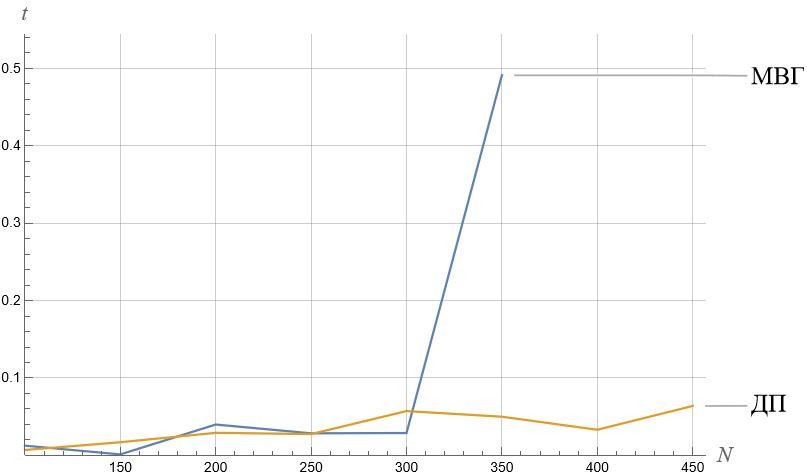
\includegraphics[scale=0.8]{plot1}
		\caption{max\_weight=1000}
	\end{figure}
	\begin{figure}[H]
		\centering
		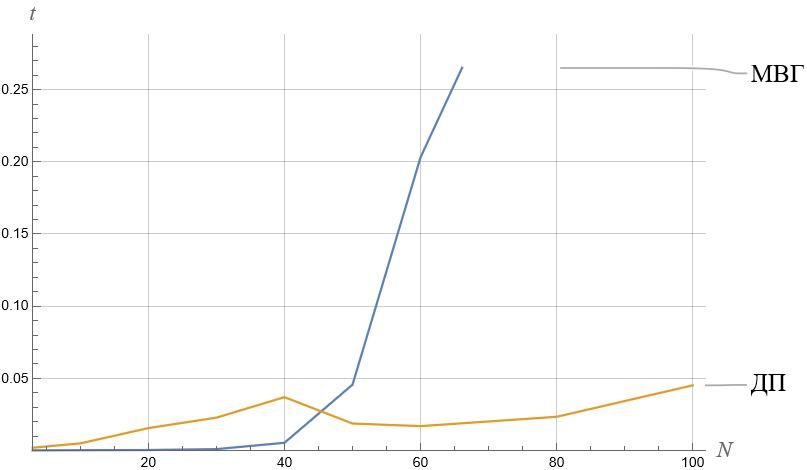
\includegraphics[scale=0.8]{plot2}
		\caption{max\_weight=3000}	
	\end{figure}	
	\begin{figure}[H]
		\centering
		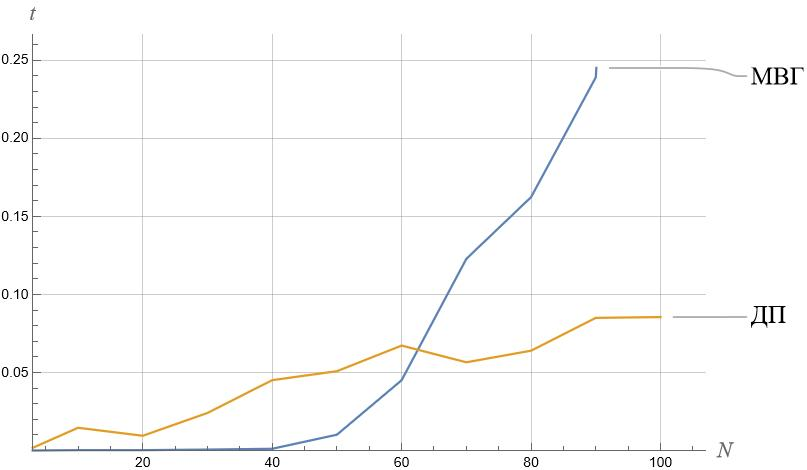
\includegraphics[scale=0.8]{plot3}
		\caption{max\_weight=5000}
	\end{figure}
	\begin{figure}[H]
		\centering
		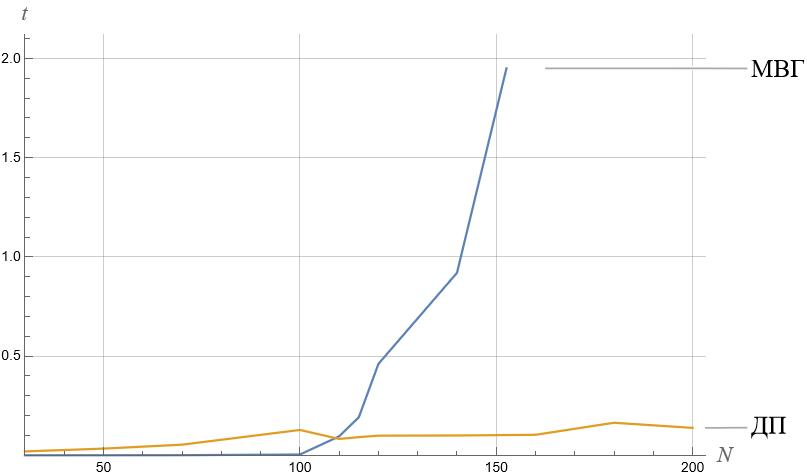
\includegraphics[scale=0.8]{plot4}
		\caption{max\_weight=10000}	
	\end{figure}	
	
	\section-{Заключение}
	В ходе практики были изучены основные возможности языка программирования C++ и системы компьютерной алгебры "Wolfram Mathematica"\,, закреплены знания и умения, полученные в рамках курсов "Введение в информационные технологии"\,, "Информационные технологии профессиональной деятельности"\,. {Были изучены методы решения задачи об ограниченном ранце. Также изучены возможности системы компьютерной алгебры "Wolfram Mathematica"\, в сфере визуализации и построения алгоритмов.
		
		\newpage
		\begin{thebibliography}{10}
			\bibitem{Kolpakov} Р.М. Колпаков, М.А. Посыпкин. Верхняя и нижняя оценки трудоемкости метода ветвей и границ для задачи о ранце, Тр. ИСА РАН, 32, 2008. C. 137---158. URL: http://www.isa.ru/proceedings/images/documents/2008-32/137-158.pdf\\(дата обращения: 23.04.2022).
			\bibitem{habr} Всё, что вы хотели знать о динамическом программировании, но боялись спросить // Хабр. [Электронный ресурс] URL: https://habr.com/ru/post/191498/.
			\bibitem{knapsack} Задача о рюкзаке // Википедия. Свободная энциклопедия. [Электронный ресурс] URL: https://ru.m.wikipedia.org/wiki/Задача\_о\_рюкзаке (дата обращения: 22.03.2022).
			\bibitem{branch and bound} Метод ветвей и границ // Википедия. Свободная энциклопедия. [Электронный ресурс] URL: https://ru.m.wikipedia.org/wiki/Метод\_ветвей\_и\_границ (дата обращения: 15.04.2022).
			\bibitem{dynamic programming} Динамическое программирование // Википедия. Свободная энциклопедия. [Электронный ресурс] URL: https://ru.m.wikipedia.org/wiki/Динамическое\_программирование (дата обращения: 25.04.2022).
			\bibitem{ITMO} Задача о рюкзаке // Университет ИТМО. [Электронный ресурс] URL: http://neerc.ifmo.ru/wiki/index.php?title=Задача\_о\_рюкзаке (дата обращения: 28.04.2022).
			\bibitem{Givens} Bounded Knapsack Algorithm [Электронный ресурс] / Givens B. URL: https://www.codeproject.com/Articles/706838/Bounded-Knapsack-Algorithm (дата обращения: 4.05.2022).
		\end{thebibliography}
		
	\end{document} 